% Queue these double-column figures before the Experiments section so they
% appear with its opening text rather than after the conclusion.
\begin{figure}[t]
    \centering
    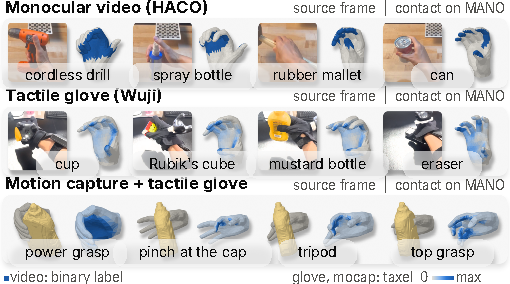
\includegraphics[width=\linewidth]{figs/fig_data_gallery_1col.pdf}
    \caption{\textbf{Demonstration sources.} We show some demonstration exmaples from monocular video (Vid-HACO contact), tactile glove (taxel pressure), and motion capture with the tactile glove  (taxel pressure).
}
    \label{fig:gallery}
\end{figure}

\begin{figure}[t]
    \centering
    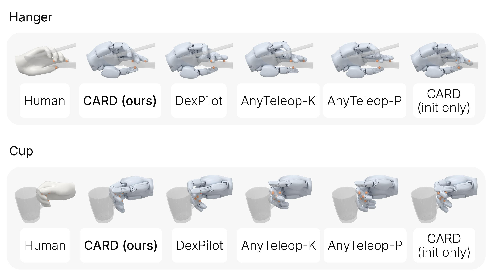
\includegraphics[width=\linewidth]{figs/fig_baselines_1col.pdf}
    \caption{\textbf{Contact-anchored vs.\ kinematic retargeting} on two video clips. Per clip: the human source, \ours, DexPilot, AnyTeleop-K, AnyTeleop-P, and \ours's geometric initialization (init only), the columns of \cref{tab:contact_quality}. The scanned object is for visualization only, and orange spheres are the \fcas. Kinematic baselines reach the object but do not track the contact.}
    \label{fig:baselines}
\end{figure}
